%%%%%%%%%%%%%%%%%%%%%%%%%%%%%%%%%%%%%%%%%
% Short Sectioned Assignment
% LaTeX Template
% Version 1.0 (5/5/12)
%
% This template has been downloaded from:
% http://www.LaTeXTemplates.com
%
% Original author:
% Frits Wenneker (http://www.howtotex.com)
%
% License:
% CC BY-NC-SA 3.0 (http://creativecommons.org/licenses/by-nc-sa/3.0/)
%
%%%%%%%%%%%%%%%%%%%%%%%%%%%%%%%%%%%%%%%%%

%----------------------------------------------------------------------------------------
%	PACKAGES AND OTHER DOCUMENT CONFIGURATIONS
%----------------------------------------------------------------------------------------

\documentclass[paper=a4, fontsize=11pt]{scrartcl} % A4 paper and 11pt font size
\usepackage{graphicx}
\usepackage[T1]{fontenc} % Use 8-bit encoding that has 256 glyphs
\usepackage{fourier} % Use the Adobe Utopia font for the document - comment this line to return to the LaTeX default
\usepackage[english]{babel} % English language/hyphenation
\usepackage{amsmath,amsfonts,amsthm} % Math packages
\usepackage{color} % This is used for highlighting text whenever you need to come back to something
\usepackage{lipsum} % Used for inserting dummy 'Lorem ipsum' text into the template
\usepackage{sectsty} % Allows customizing section commands
\allsectionsfont{\centering \normalfont\scshape} % Make all sections centered, the default font and small caps
\usepackage{fancyhdr} % Custom headers and footers
\pagestyle{fancyplain} % Makes all pages in the document conform to the custom headers and footers
\fancyhead{} % No page header - if you want one, create it in the same way as the footers below
\fancyfoot[L]{} % Empty left footer
\fancyfoot[C]{} % Empty center footer
\fancyfoot[R]{\thepage} % Page numbering for right footer
\renewcommand{\headrulewidth}{0pt} % Remove header underlines
\renewcommand{\footrulewidth}{0pt} % Remove footer underlines
\setlength{\headheight}{13.6pt} % Customize the height of the header

%numberwithin{equation}{section} % Number equations within sections (i.e. 1.1, 1.2, 2.1, 2.2 instead of 1, 2, 3, 4)
%\numberwithin{figure}{section} % Number figures within sections (i.e. 1.1, 1.2, 2.1, 2.2 instead of 1, 2, 3, 4)
%\numberwithin{table}{section} % Number tables within sections (i.e. 1.1, 1.2, 2.1, 2.2 instead of 1, 2, 3, 4)

%\setlength\parindent{0pt} % Removes all indentation from paragraphs - comment this line for an assignment with lots of text

%----------------------------------------------------------------------------------------
%	TITLE SECTION
%----------------------------------------------------------------------------------------

\newcommand{\horrule}[1]{\rule{\linewidth}{#1}} % Create horizontal rule command with 1 argument of height

\title{	
\normalfont \normalsize 
\textsc{Columbia University -- CUNY} \\ [25pt] % Your university, school and/or department name(s)
\horrule{0.5pt} \\[0.4cm] % Thin top horizontal rule
\huge Homework 2 - NLP/ML/Web \\ % The assignment title
\horrule{2pt} \\[0.5cm] % Thick bottom horizontal rule
}

\author{Jessica Ouyang and Joe Ellis} % Your name

\date{\normalsize\today} % Today's date or a custom date

\begin{document}

\maketitle % Print the title

%---
% Task 
%---

\section{Task -- Language Modeling}
\paragraph{}
In this problem we are tasked with attempting to modeling a language example of at least 100,000 words and another language model that is created using a seperate corpus of at least 50,000 words.  For this experiment we chose to use two famous novels as our language examples, one being ``The Scarlet Letter'' by Nathaniel Hawthorne and the other being ``A Tale of Two Cities'' written by Charles Dickens.  Both were modeled using different n-gram language models.  We also applied Laplacian smoothing and back-off to our models to create more accuracte language models.  Finally, we created a combined model trained off of both language examples.

\section{Experiments and Results}
\subsection{Task 1 -- Domain A}


\paragraph{1a -- Download Language Text}
For our first domain we chose to download and use the famous novel ``A Tale of Two Cities'' by Charles Dickens.  The novel had much more than 100,000 words.  For our train and test split we decided that we would use 60\% of the available data for test, 20\% for development, and 20\% for evalauation.

\paragraph{1b - Find N for Language Model}
After this we had to find the N for the N gram model that would be utilized for this text.  The best result in our examples for the proper N-gram model was the tri-gram model.  This first example we did not do any smoothing, therefore we evaluated only on the seen grams from the development set, and chose N that provided the lowest perplexity.  Average Perplexity per gram was calculated using the formula,

\begin{align}
Perplexity_{ave}(text) = 2^{-\frac{1}{N}\sum_1^N p(w_i)log(p(w_i))}
\end{align}

We chose to use this formula, so that different models with differing data sizes can be compared $x$.
We chose tri-gram as the best model, and the graph of the results can be seen in Figure ~ref{fig:figure1}.  The results on the test set for seen grams is $Perplexity(test)=15.426$

\begin{figure}
\centering
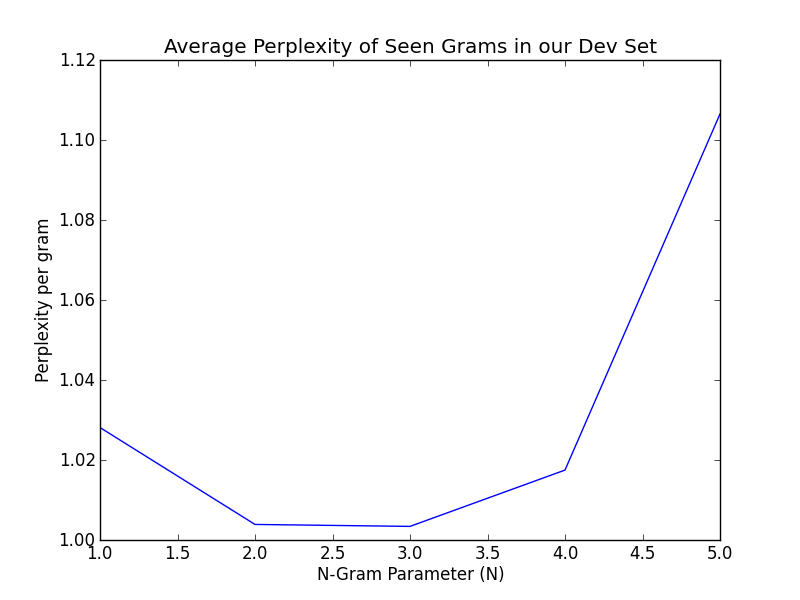
\includegraphics[scale=0.4]{figure_1.png}
\caption{N-Gram Performance for Domain A}
\label{fig:figure1}
\end{figure}

\paragraph{1c -- Laplace Smoothing}
We also utilized Laplace smoothing to solve for the best value of N with Laplace Smoothing utilized.  When we use Laplace smoothing instead of using simply $p(w)=\frac{N(w)}{N}$, we include and extra value of $V$ into the equation where $V$ is the number of distinct N-grams present.  Therefore, the new $p(w) = \frac{N(w)+1}{N+V}$.  This allows us to classify all of the values seen, but gives small probablities to unseen before grams.  The results of this modeling scheme can be seen below, and for this model tri-gram also wins out.  
However, since many of the n-grams are unseen for $n=4$ or $n=5$, the penalty is not as high as before.  The results are shown in Figure ~\ref{fig:figure2}.  
The result on the test set for all grams with smoothing is,  $Perplexity(test)=2^{-31.25}$, and the total entropy is $-31.250$.

\begin{figure}
\centering
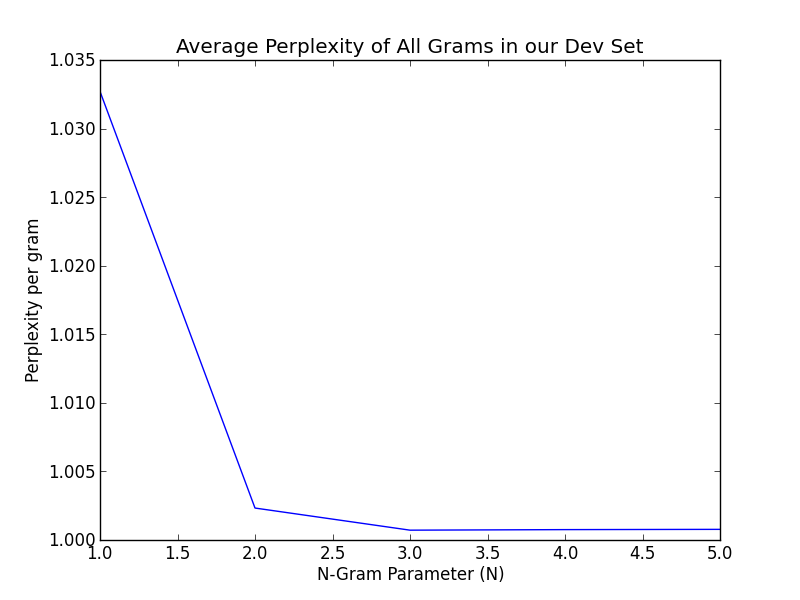
\includegraphics[scale=0.4]{figure_2.png}
\caption{N-Gram Performance for Domain A}
\label{fig:figure2}
\end{figure}

\paragraph{1d -- Back-Off}
Finally, we addressed the issue of unseen grams during training using the Back-Off parameters.  For, Back-Off we use $p(w)$ as a linear interpolation of the values of each condition probablity that makes up $p(w)$.  Therefore, the equation for back-off is as follows,

\begin{align}
p(w)=\lambda_0p(w_0) + \lambda_1p(w_1|w_0) + \lambda_2p(w_2|w_1,w_0).
\end{align}

We would have used 4-gram for back-off training, however once I got to 4-gram language representation 98\% of my grams were unseen.  
So most of the values would be unseen for this case, and therefore we chose to only perform back-off from 3.
We attempted to use a variety of different lambdas for the language model and the results can be seen below in Table ~ref{tab:table1}.  We have chosen our $\lambda$ wieghting scheme as $\lambda=(0.0,0.3,0.7)$, and this is because we wanted all $\lambda$s to be non-zero, but the unigram model was not useful for this problem. The perplexity score on our test dataset using these parameters was $Perplexity(test) = 2^{241.31}$.  

\begin{table}
\centering
\label{tab:table1}
\caption{lambda values and perplexity scores}
\begin{tabular}{|c|c|c|c|}
\hline
$\lambda_0$ & $\lambda_1$ & $\lambda_2$ & $Perplexity_{ave}(dev)$ \\ \hline \hline
0 & 0.5 & 0.5 & 1.0075  \\ \hline
0.33 & 0.33 & 0.33 & 1.0181 \\ \hline
0.2 & 0.4 & 0.4 & 1.0145 \\ \hline
0.5 & 0.25 & 0.25 & 1.0223 \\ \hline
0.25 & 0.5 & 0.25 & 1.0171 \\ \hline
0.25 & 0.25 & 0.5 & 1.0148 \\ \hline
0.1 & 0.2 & 0.7 & 1.0089 \\ \hline
0.0 & 0.3 & 0.7 & 1.0055 \\ \hline
\end{tabular}
\end{table}

\subsection{Task 2}
\paragraph{2a - Download another Domain}
For our second domain, we utilized the famous novel ``The Scarlet Letter'' by Nathaniel Hawthorne.  This book contains over 50,000 words and the train and test split of the data was the same as was used above.

\paragraph{2b - Find Optimal Language Model}
The same tests were used as those described above to find the optimal language model for this text, and we received similar results.  Once again the highest performing model was the tri-gram model with smoothing.  This model appears to work well on many datasets, however it would be useful to have more training data as many of the grams remain unseen even in this model.  The perplexity of this model on the test-set on the seen grams is $Perplexity(test)=2^{0.2627}=1.2033$.  When we utilized the $\lambda=(0.0,0.6,0.4)$ parameters and performed back-off ad smoothing on the set we received a perplexity score on our dataset of $Perplexity(test)=2^{113.5347}$

\paragraph{2c-Cross Domain Analysis}
We also attempted to see how our first domain model, the model that was trained on Dickens performed on The Scarlet Letter.  The performance was similar but slightly degraded, and the resulting average entropy per n-gram is $-0.0120$, which over the 18,652 trigrams testsed gives us  a perplexity of, $Perplexity(crossdomain) = 2^{108.0305}$.

\paragraph{2d- Interpolated Model}
Finally, we also tested on the The Scarlet Letter an interpolated model, that allowed for us to utilized both trained models for modeling.  For this model we linearly combined the probablilty received from both models using $\lambda$ parameters and the results on the development set can be seen below for multiple $\lambda$.  We have $\lambda_0$ corresponding to ``A Tale of Two Cities'' trained model and $\lambda_1$ corresponds to ``The Scarlet Letter'' trained model.  
These values outperform just the Scarlet Letter Model by itself on the test data, greatly.

\begin{table}
\centering
\label{tab:table2}
\caption{lambda values and perplexity scores for linearly combined model}
\begin{tabular}{|c|c|c|}
\hline
$\lambda_0$ & $\lambda_1$ & $Perplexity(dev)$ \\ \hline \hline
0.5 & 0.5 & $2^{88.62}$ \\ \hline
0.2 & 0.8 & $2^{84.42}$ \\ \hline
0.3 & 0.7 & $2^{85.88}$ \\ \hline
\end{tabular}
\end{table}

\paragraph{2e - Interpolated Model Performance}
The testing was performed on the ``The Scarlet Letter'' test set, and the resulting perplexity using interpolation parameters $(\lambda_{int} = (0.2,0.7)$ is $Perplexity(test) = 2^{77.39}$.  This shows just how useful it is to have multiple models and broaden our training data.  The interpolated model outperforms both singluar models by itself.

\section{Linguistic Oriented Section}

\end{document}